% Options for packages loaded elsewhere
\PassOptionsToPackage{unicode}{hyperref}
\PassOptionsToPackage{hyphens}{url}
\documentclass[
  russian,
]{article}
\usepackage{xcolor}
\usepackage[margin=20mm]{geometry}
\usepackage{amsmath,amssymb}
\setcounter{secnumdepth}{-\maxdimen} % remove section numbering
\usepackage{iftex}
\ifPDFTeX
  \usepackage[T1]{fontenc}
  \usepackage[utf8]{inputenc}
  \usepackage{textcomp} % provide euro and other symbols
\else % if luatex or xetex
  \usepackage{unicode-math} % this also loads fontspec
  \defaultfontfeatures{Scale=MatchLowercase}
  \defaultfontfeatures[\rmfamily]{Ligatures=TeX,Scale=1}
\fi
\usepackage{lmodern}
\ifPDFTeX\else
  % xetex/luatex font selection
  \setmainfont[]{Arial Unicode MS}
  \setmonofont[]{Menlo}
\fi
% Use upquote if available, for straight quotes in verbatim environments
\IfFileExists{upquote.sty}{\usepackage{upquote}}{}
\IfFileExists{microtype.sty}{% use microtype if available
  \usepackage[]{microtype}
  \UseMicrotypeSet[protrusion]{basicmath} % disable protrusion for tt fonts
}{}
\makeatletter
\@ifundefined{KOMAClassName}{% if non-KOMA class
  \IfFileExists{parskip.sty}{%
    \usepackage{parskip}
  }{% else
    \setlength{\parindent}{0pt}
    \setlength{\parskip}{6pt plus 2pt minus 1pt}}
}{% if KOMA class
  \KOMAoptions{parskip=half}}
\makeatother
\usepackage{color}
\usepackage{fancyvrb}
\newcommand{\VerbBar}{|}
\newcommand{\VERB}{\Verb[commandchars=\\\{\}]}
\DefineVerbatimEnvironment{Highlighting}{Verbatim}{commandchars=\\\{\}}
% Add ',fontsize=\small' for more characters per line
\newenvironment{Shaded}{}{}
\newcommand{\AlertTok}[1]{\textcolor[rgb]{1.00,0.00,0.00}{\textbf{#1}}}
\newcommand{\AnnotationTok}[1]{\textcolor[rgb]{0.38,0.63,0.69}{\textbf{\textit{#1}}}}
\newcommand{\AttributeTok}[1]{\textcolor[rgb]{0.49,0.56,0.16}{#1}}
\newcommand{\BaseNTok}[1]{\textcolor[rgb]{0.25,0.63,0.44}{#1}}
\newcommand{\BuiltInTok}[1]{\textcolor[rgb]{0.00,0.50,0.00}{#1}}
\newcommand{\CharTok}[1]{\textcolor[rgb]{0.25,0.44,0.63}{#1}}
\newcommand{\CommentTok}[1]{\textcolor[rgb]{0.38,0.63,0.69}{\textit{#1}}}
\newcommand{\CommentVarTok}[1]{\textcolor[rgb]{0.38,0.63,0.69}{\textbf{\textit{#1}}}}
\newcommand{\ConstantTok}[1]{\textcolor[rgb]{0.53,0.00,0.00}{#1}}
\newcommand{\ControlFlowTok}[1]{\textcolor[rgb]{0.00,0.44,0.13}{\textbf{#1}}}
\newcommand{\DataTypeTok}[1]{\textcolor[rgb]{0.56,0.13,0.00}{#1}}
\newcommand{\DecValTok}[1]{\textcolor[rgb]{0.25,0.63,0.44}{#1}}
\newcommand{\DocumentationTok}[1]{\textcolor[rgb]{0.73,0.13,0.13}{\textit{#1}}}
\newcommand{\ErrorTok}[1]{\textcolor[rgb]{1.00,0.00,0.00}{\textbf{#1}}}
\newcommand{\ExtensionTok}[1]{#1}
\newcommand{\FloatTok}[1]{\textcolor[rgb]{0.25,0.63,0.44}{#1}}
\newcommand{\FunctionTok}[1]{\textcolor[rgb]{0.02,0.16,0.49}{#1}}
\newcommand{\ImportTok}[1]{\textcolor[rgb]{0.00,0.50,0.00}{\textbf{#1}}}
\newcommand{\InformationTok}[1]{\textcolor[rgb]{0.38,0.63,0.69}{\textbf{\textit{#1}}}}
\newcommand{\KeywordTok}[1]{\textcolor[rgb]{0.00,0.44,0.13}{\textbf{#1}}}
\newcommand{\NormalTok}[1]{#1}
\newcommand{\OperatorTok}[1]{\textcolor[rgb]{0.40,0.40,0.40}{#1}}
\newcommand{\OtherTok}[1]{\textcolor[rgb]{0.00,0.44,0.13}{#1}}
\newcommand{\PreprocessorTok}[1]{\textcolor[rgb]{0.74,0.48,0.00}{#1}}
\newcommand{\RegionMarkerTok}[1]{#1}
\newcommand{\SpecialCharTok}[1]{\textcolor[rgb]{0.25,0.44,0.63}{#1}}
\newcommand{\SpecialStringTok}[1]{\textcolor[rgb]{0.73,0.40,0.53}{#1}}
\newcommand{\StringTok}[1]{\textcolor[rgb]{0.25,0.44,0.63}{#1}}
\newcommand{\VariableTok}[1]{\textcolor[rgb]{0.10,0.09,0.49}{#1}}
\newcommand{\VerbatimStringTok}[1]{\textcolor[rgb]{0.25,0.44,0.63}{#1}}
\newcommand{\WarningTok}[1]{\textcolor[rgb]{0.38,0.63,0.69}{\textbf{\textit{#1}}}}
\usepackage{longtable,booktabs,array}
\newcounter{none} % for unnumbered tables
\usepackage{calc} % for calculating minipage widths
% Correct order of tables after \paragraph or \subparagraph
\usepackage{etoolbox}
\makeatletter
\patchcmd\longtable{\par}{\if@noskipsec\mbox{}\fi\par}{}{}
\makeatother
% Allow footnotes in longtable head/foot
\IfFileExists{footnotehyper.sty}{\usepackage{footnotehyper}}{\usepackage{footnote}}
\makesavenoteenv{longtable}
\usepackage{graphicx}
\makeatletter
\newsavebox\pandoc@box
\newcommand*\pandocbounded[1]{% scales image to fit in text height/width
  \sbox\pandoc@box{#1}%
  \Gscale@div\@tempa{\textheight}{\dimexpr\ht\pandoc@box+\dp\pandoc@box\relax}%
  \Gscale@div\@tempb{\linewidth}{\wd\pandoc@box}%
  \ifdim\@tempb\p@<\@tempa\p@\let\@tempa\@tempb\fi% select the smaller of both
  \ifdim\@tempa\p@<\p@\scalebox{\@tempa}{\usebox\pandoc@box}%
  \else\usebox{\pandoc@box}%
  \fi%
}
% Set default figure placement to htbp
\def\fps@figure{htbp}
\makeatother
\ifLuaTeX
\usepackage[bidi=basic,shorthands=off,provide=*]{babel}
\else
\usepackage[bidi=default,shorthands=off,provide=*]{babel}
\fi
\ifPDFTeX
\else
\babelfont{rm}[]{Arial Unicode MS}
\fi
\ifLuaTeX
  \usepackage{selnolig} % disable illegal ligatures
\fi
\setlength{\emergencystretch}{3em} % prevent overfull lines
\providecommand{\tightlist}{%
  \setlength{\itemsep}{0pt}\setlength{\parskip}{0pt}}
\usepackage{bookmark}
\IfFileExists{xurl.sty}{\usepackage{xurl}}{} % add URL line breaks if available
\urlstyle{same}
\hypersetup{
  pdftitle={Лабораторная работа № 3},
  pdflang={ru-RU},
  hidelinks,
  pdfcreator={LaTeX via pandoc}}

\title{Лабораторная работа № 3}
\usepackage{etoolbox}
\makeatletter
\providecommand{\subtitle}[1]{% add subtitle to title
  \apptocmd{\@title}{\par {\large #1 \par}}{}{}
}
\makeatother
\subtitle{Исследование конвейера SCR1. Вариант 9: DIV}
\author{}
\date{}

\begin{document}
\begin{titlepage}
\newgeometry{left=20mm,right=20mm,top=20mm,bottom=20mm}
\thispagestyle{empty}
\begingroup
\fontspec{Times New Roman}
\fontsize{14}{25}\selectfont
\begin{center}
Федеральное государственное автономное\\
образовательное учреждение высшего образования\\
«Национальный исследовательский университет ИТМО»

\vspace{10mm}
Факультет программной инженерии и компьютерной техники

\vspace{34mm}
\textbf{ОТЧЁТ}\\
по лабораторной работе № 3\\
по дисциплине «Проектирование систем на кристалле»\\
«Анализ выполнения инструкции DIV в конвейере SCR1»\\
Вариант 9
\end{center}

\vspace{43mm}
\begin{flushright}
Выполнила:\\
Пронина Анастасия Ильинична\\
Группа: P4130
\end{flushright}

\vfill
\begin{center}
Санкт-Петербург\\
2026
\end{center}
\endgroup
\end{titlepage}
\restoregeometry
\setcounter{page}{2}

\section{1. Цель и
задание}\label{ux446ux435ux43bux44c-ux438-ux437ux430ux434ux430ux43dux438ux435}

Изучить выполнение инструкции знакового целочисленного деления DIV в
конвейере SCR1. Добавить несинтезируемый наблюдатель, выводящий атрибуты
команды, и исследовать её выполнение по временной диаграмме.

Вариант 9: инструкция \texttt{div}; отладочная информация --- значения
атрибутов команды. Рабочая ветка --- \texttt{lab3\_scr1\_pipe\_analys}.

\section{2. Окружение и
запуск}\label{ux43eux43aux440ux443ux436ux435ux43dux438ux435-ux438-ux437ux430ux43fux443ux441ux43a}

Использовано Docker-окружение проекта, Verilator 5.030, интерфейс AHB и
конфигурация MAX (RV32IMC). Для анализа записана VCD-трасса с текстовой
трассировкой.

В \texttt{sim/tests/riscv\_isa/rv32\_tests.inc} оставлен единственный
тест:

\begin{Shaded}
\begin{Highlighting}[]
\NormalTok{rv32\_isa\_tests := isa/rv32um/div.S}
\end{Highlighting}
\end{Shaded}

Команда запуска внутри контейнера, из \texttt{/work/scr1}:

\begin{Shaded}
\begin{Highlighting}[]
\FunctionTok{make}\NormalTok{ run\_verilator\_wf CFG=MAX BUS=AHB TARGETS=riscv\_isa TRACE=1}
\end{Highlighting}
\end{Shaded}

Результаты находятся в
\texttt{build/verilator\_wf\_AHB\_MAX\_imc\_IPIC\_1\_TCM\_1\_VIRQ\_1\_TRACE\_1/}.
Файлы \texttt{div.dump}, \texttt{simx.vcd} и \texttt{test\_results.txt}
использованы для проверки адресов, времён и результата теста.


\subsection*{2.1. Последовательность выполненных действий}

\begin{enumerate}
\item \textbf{Подготовлена рабочая ветка.}
Работа ведётся в отдельной ветке \texttt{lab3\_scr1\_pipe\_analys}
репозитория SCR1. Её исходный коммит --- \texttt{ebb5e35}.
Удалённый \texttt{origin} настроен на личный репозиторий
\url{https://github.com/ProshkaAnastasia/scr1}; для отправки используется SSH.
Реализация лабораторной зафиксирована коммитом \texttt{60646bb}\newline
(\texttt{Add simulation}); ветка с реализацией отправлена в личный репозиторий.

\item \textbf{Выбран тест по варианту.}
Из списка ISA-тестов удалены остальные тесты и условные добавления
наборов M/C. Оставлена только строка с \texttt{isa/rv32um/div.S}.
Выбор \texttt{CFG=MAX} обеспечивает поддержку расширения M,
необходимого для DIV; редактировать декодер для включения деления не требовалось.

\item \textbf{Получена первоначальная диаграмма.}
Симуляция запущена с целью \texttt{run\_verilator\_wf} и параметром
\texttt{TRACE=1}. Найден файл \texttt{simx.vcd}, открытый в GTKWave
на macOS; сама модель выполнялась в Docker.

\item \textbf{Изучен путь команды в исходниках.}
В IDU найдена ветвь регистровых операций расширения M, выбирающая
\texttt{SCR1\_IALU\_CMD\_DIV}. В EXU прослежены приём команды,
чтение MPRF, подключение IALU, готовность и запись результата.
В \texttt{div.dump} выбран адрес первой DIV --- \texttt{0x2A8}.

\item \textbf{Добавлен отладочный модуль.}
Создан \texttt{src/tb/scr1\_tb\_log\_cmd.sv}.
Его экземпляр \texttt{i\_log\_cmd} подключён в AHB-тестбенче,
а исходник добавлен в \texttt{src/ahb\_tb.files}.
Модуль наблюдает завершение DIV по действующей команде и разрешению
записи. Процессор не создаётся повторно: используются сигналы уже
существующего экземпляра EXU.

\item \textbf{Выполнена повторная симуляция с наблюдателем.}
После включения нового модуля сборка и запуск повторены.
Получены девять сообщений \texttt{[DIV]}, результат
\texttt{div.hex: OK, PASS} и итог \texttt{1/1 tests passed}.
Адреса сообщений сопоставлены с дизассемблированием;
значения результатов проверены, включая особые случаи.

\item \textbf{Настроены сигналы GTKWave.}
Такт взят с верхнего уровня или из EXU, текущий PC --- из EXU
(\texttt{pc\_i} наблюдателя), а четыре сигнала памяти инструкций ---
из \texttt{i\_top.i\_imem\_ahb}.
Дополнительно выведены значения операндов, номера регистров,
достоверность команды, разрешение записи и результат.
Выбран интервал, включающий поступление DIV в EXU и запись частного.

\item \textbf{Сохранены материалы анализа.}
Скриншот GTKWave сохранён в \texttt{diagram.png}, текстовый вывод ---
в \texttt{div\_debug.log}, результат теста --- в
\texttt{test\_results.txt}. Скриншот включён в данный отчёт с обрезкой;
дополнительно приведены поясняющие рисунки из той же VCD-трассы.
\end{enumerate}

\section{3. Изменения в
проекте}\label{ux438ux437ux43cux435ux43dux435ux43dux438ux44f-ux432-ux43fux440ux43eux435ux43aux442ux435}

{\def\LTcaptype{none} % do not increment counter
\begin{longtable}[]{@{}
  >{\raggedright\arraybackslash}p{(\linewidth - 2\tabcolsep) * \real{0.5000}}
  >{\raggedright\arraybackslash}p{(\linewidth - 2\tabcolsep) * \real{0.5000}}@{}}
\toprule\noalign{}
\begin{minipage}[b]{\linewidth}\raggedright
Файл
\end{minipage} & \begin{minipage}[b]{\linewidth}\raggedright
Изменение
\end{minipage} \\
\midrule\noalign{}
\endhead
\bottomrule\noalign{}
\endlastfoot
\texttt{sim/tests/riscv\_isa/rv32\_tests.inc} & Выбран только тест
\texttt{div.S}. \\
\texttt{src/tb/scr1\_tb\_log\_cmd.sv} & Добавлен наблюдатель исполнения
DIV. \\
\texttt{src/ahb\_tb.files} & Наблюдатель включён в список исходников. \\
\texttt{src/tb/scr1\_top\_tb\_ahb.sv} & Создан экземпляр наблюдателя и
подключены сигналы EXU. \\
\end{longtable}
}

Процессорное RTL не изменялось для добавления наблюдателя. Код вывода
размещён в тестовом окружении и ограничен директивами
\texttt{synthesis\ translate\_off/on}.

\section{4. Устройство
наблюдателя}\label{ux443ux441ux442ux440ux43eux439ux441ux442ux432ux43e-ux43dux430ux431ux43bux44eux434ux430ux442ux435ux43bux44f}

Модуль не загружает программу и не выполняет деление. Он получает
сигналы экземпляра
\texttt{i\_top.i\_core\_top.i\_pipe\_top.i\_pipe\_exu} и наблюдает
завершение инструкции.

{\def\LTcaptype{none} % do not increment counter
\begin{longtable}[]{@{}
  >{\raggedright\arraybackslash}p{(\linewidth - 4\tabcolsep) * \real{0.3333}}
  >{\raggedright\arraybackslash}p{(\linewidth - 4\tabcolsep) * \real{0.3333}}
  >{\raggedright\arraybackslash}p{(\linewidth - 4\tabcolsep) * \real{0.3333}}@{}}
\toprule\noalign{}
\begin{minipage}[b]{\linewidth}\raggedright
Вход наблюдателя
\end{minipage} & \begin{minipage}[b]{\linewidth}\raggedright
Сигнал EXU
\end{minipage} & \begin{minipage}[b]{\linewidth}\raggedright
Смысл
\end{minipage} \\
\midrule\noalign{}
\endhead
\bottomrule\noalign{}
\endlastfoot
\texttt{clk}, \texttt{rst\_n} & \texttt{clk}, \texttt{rst\_n} & Такт и
сброс. \\
\texttt{valid\_i} & \texttt{exu\_queue\_vd} & Текущая команда
достоверна. \\
\texttt{cmd\_i} & \texttt{exu\_queue} & Декодированная операция и номера
регистров. \\
\texttt{pc\_i} & \texttt{pc\_curr\_ff} & PC стадии исполнения. \\
\texttt{operand1\_i}, \texttt{operand2\_i} & \texttt{ialu\_main\_op1},
\texttt{ialu\_main\_op2} & Делимое и делитель. \\
\texttt{writeback\_i} & \texttt{exu2mprf\_w\_req\_o} & Разрешена запись
результата. \\
\texttt{result\_i} & \texttt{exu2mprf\_rd\_data\_o} & Данные для записи
в регистр. \\
\end{longtable}
}

На положительном фронте такта проверяется:

\begin{Shaded}
\begin{Highlighting}[]
\NormalTok{rst\_n \&\& valid\_i \&\& writeback\_i}
\NormalTok{    \&\& (cmd\_i.ialu\_cmd == SCR1\_IALU\_CMD\_DIV)}
\end{Highlighting}
\end{Shaded}

Это позволяет печатать одно сообщение при записи результата каждой
завершённой DIV, вместо повторения на каждом такте многотактного
вычисления. Выводятся PC, номера \texttt{rs1}, \texttt{rs2},
\texttt{rd}, значения операндов и результат. Приведение
\texttt{\$signed} обеспечивает знаковое десятичное представление.

\texttt{valid\_i} не означает завершение команды: он остаётся
установленным во время исполнения. \texttt{writeback\_i} означает
разрешение записи на фронте. При последовательности однотактных команд
разрешение может оставаться единицей несколько тактов, обслуживая разные
инструкции.

\section{5. Прохождение DIV через
конвейер}\label{ux43fux440ux43eux445ux43eux436ux434ux435ux43dux438ux435-div-ux447ux435ux440ux435ux437-ux43aux43eux43dux432ux435ux439ux435ux440}

\begin{enumerate}
\def\labelenumi{\arabic{enumi}.}
\tightlist
\item
  IFU выбирает машинное слово из памяти инструкций и передаёт его IDU.
\item
  IDU распознаёт \texttt{opcode\ =\ 0110011},
  \texttt{funct7\ =\ 0000001}, \texttt{funct3\ =\ 100} как DIV. Он
  формирует \texttt{SCR1\_IALU\_CMD\_DIV}, выбирает два регистровых
  операнда и результат IALU для записи в \texttt{rd}.
\item
  При готовности EXU команда сохраняется в \texttt{exu\_queue}. Из MPRF
  читаются значения регистров-источников. В используемой реализации MPRF
  чтение комбинационное, запись --- по фронту.
\item
  IALU выполняет итерационное деление. Пока результат не готов, EXU
  удерживает текущую команду и не принимает следующую в свой буфер.
\item
  При готовности частного разрешается запись. На положительном фронте
  MPRF фиксирует результат; при обычном продолжении PC увеличивается на
  4.
\end{enumerate}

Для первой проверки исходник содержит
\texttt{TEST\_RR\_OP(2,\ div,\ 3,\ 20,\ 6)}. В дизассемблировании:

\begin{Shaded}
\begin{Highlighting}[]
\NormalTok{2a0: 01400093  li  ra,20}
\NormalTok{2a4: 00600113  li  sp,6}
\NormalTok{2a8: 0220c1b3  div gp,ra,sp}
\NormalTok{2ac: 00300e93  li  t4,3}
\NormalTok{2b0: 00200e13  li  t3,2}
\NormalTok{2b4: 0dd19463  bne gp,t4,37c \textless{}fail\textgreater{}}
\end{Highlighting}
\end{Shaded}

Здесь \texttt{ra=x1}, \texttt{sp=x2}, \texttt{gp=x3}, \texttt{t4=x29},
\texttt{t3=x28}. Деление записывает частное в x3. Затем тест сравнивает
x3 с эталоном 3; при несовпадении выполняется переход на \texttt{fail}.

\section{6. Временные
диаграммы}\label{ux432ux440ux435ux43cux435ux43dux43dux44bux435-ux434ux438ux430ux433ux440ux430ux43cux43cux44b}

Ниже приведён скриншот GTKWave и поясняющие диаграммы, построенные
непосредственно по изменениям сигналов \texttt{simx.vcd}. Скриншот
обрезан средствами LaTeX: сохранены названия сигналов, шкала времени
и графики; дерево модулей и пустая нижняя область скрыты.
Исходный файл \texttt{diagram.png} не изменён.

\begin{figure}[htbp]
\centering
% Исходник: 3024 x 1890 пикселей, 144 dpi; trim указан в bp (72 на дюйм).
% Порядок обрезки: слева, снизу, справа, сверху.
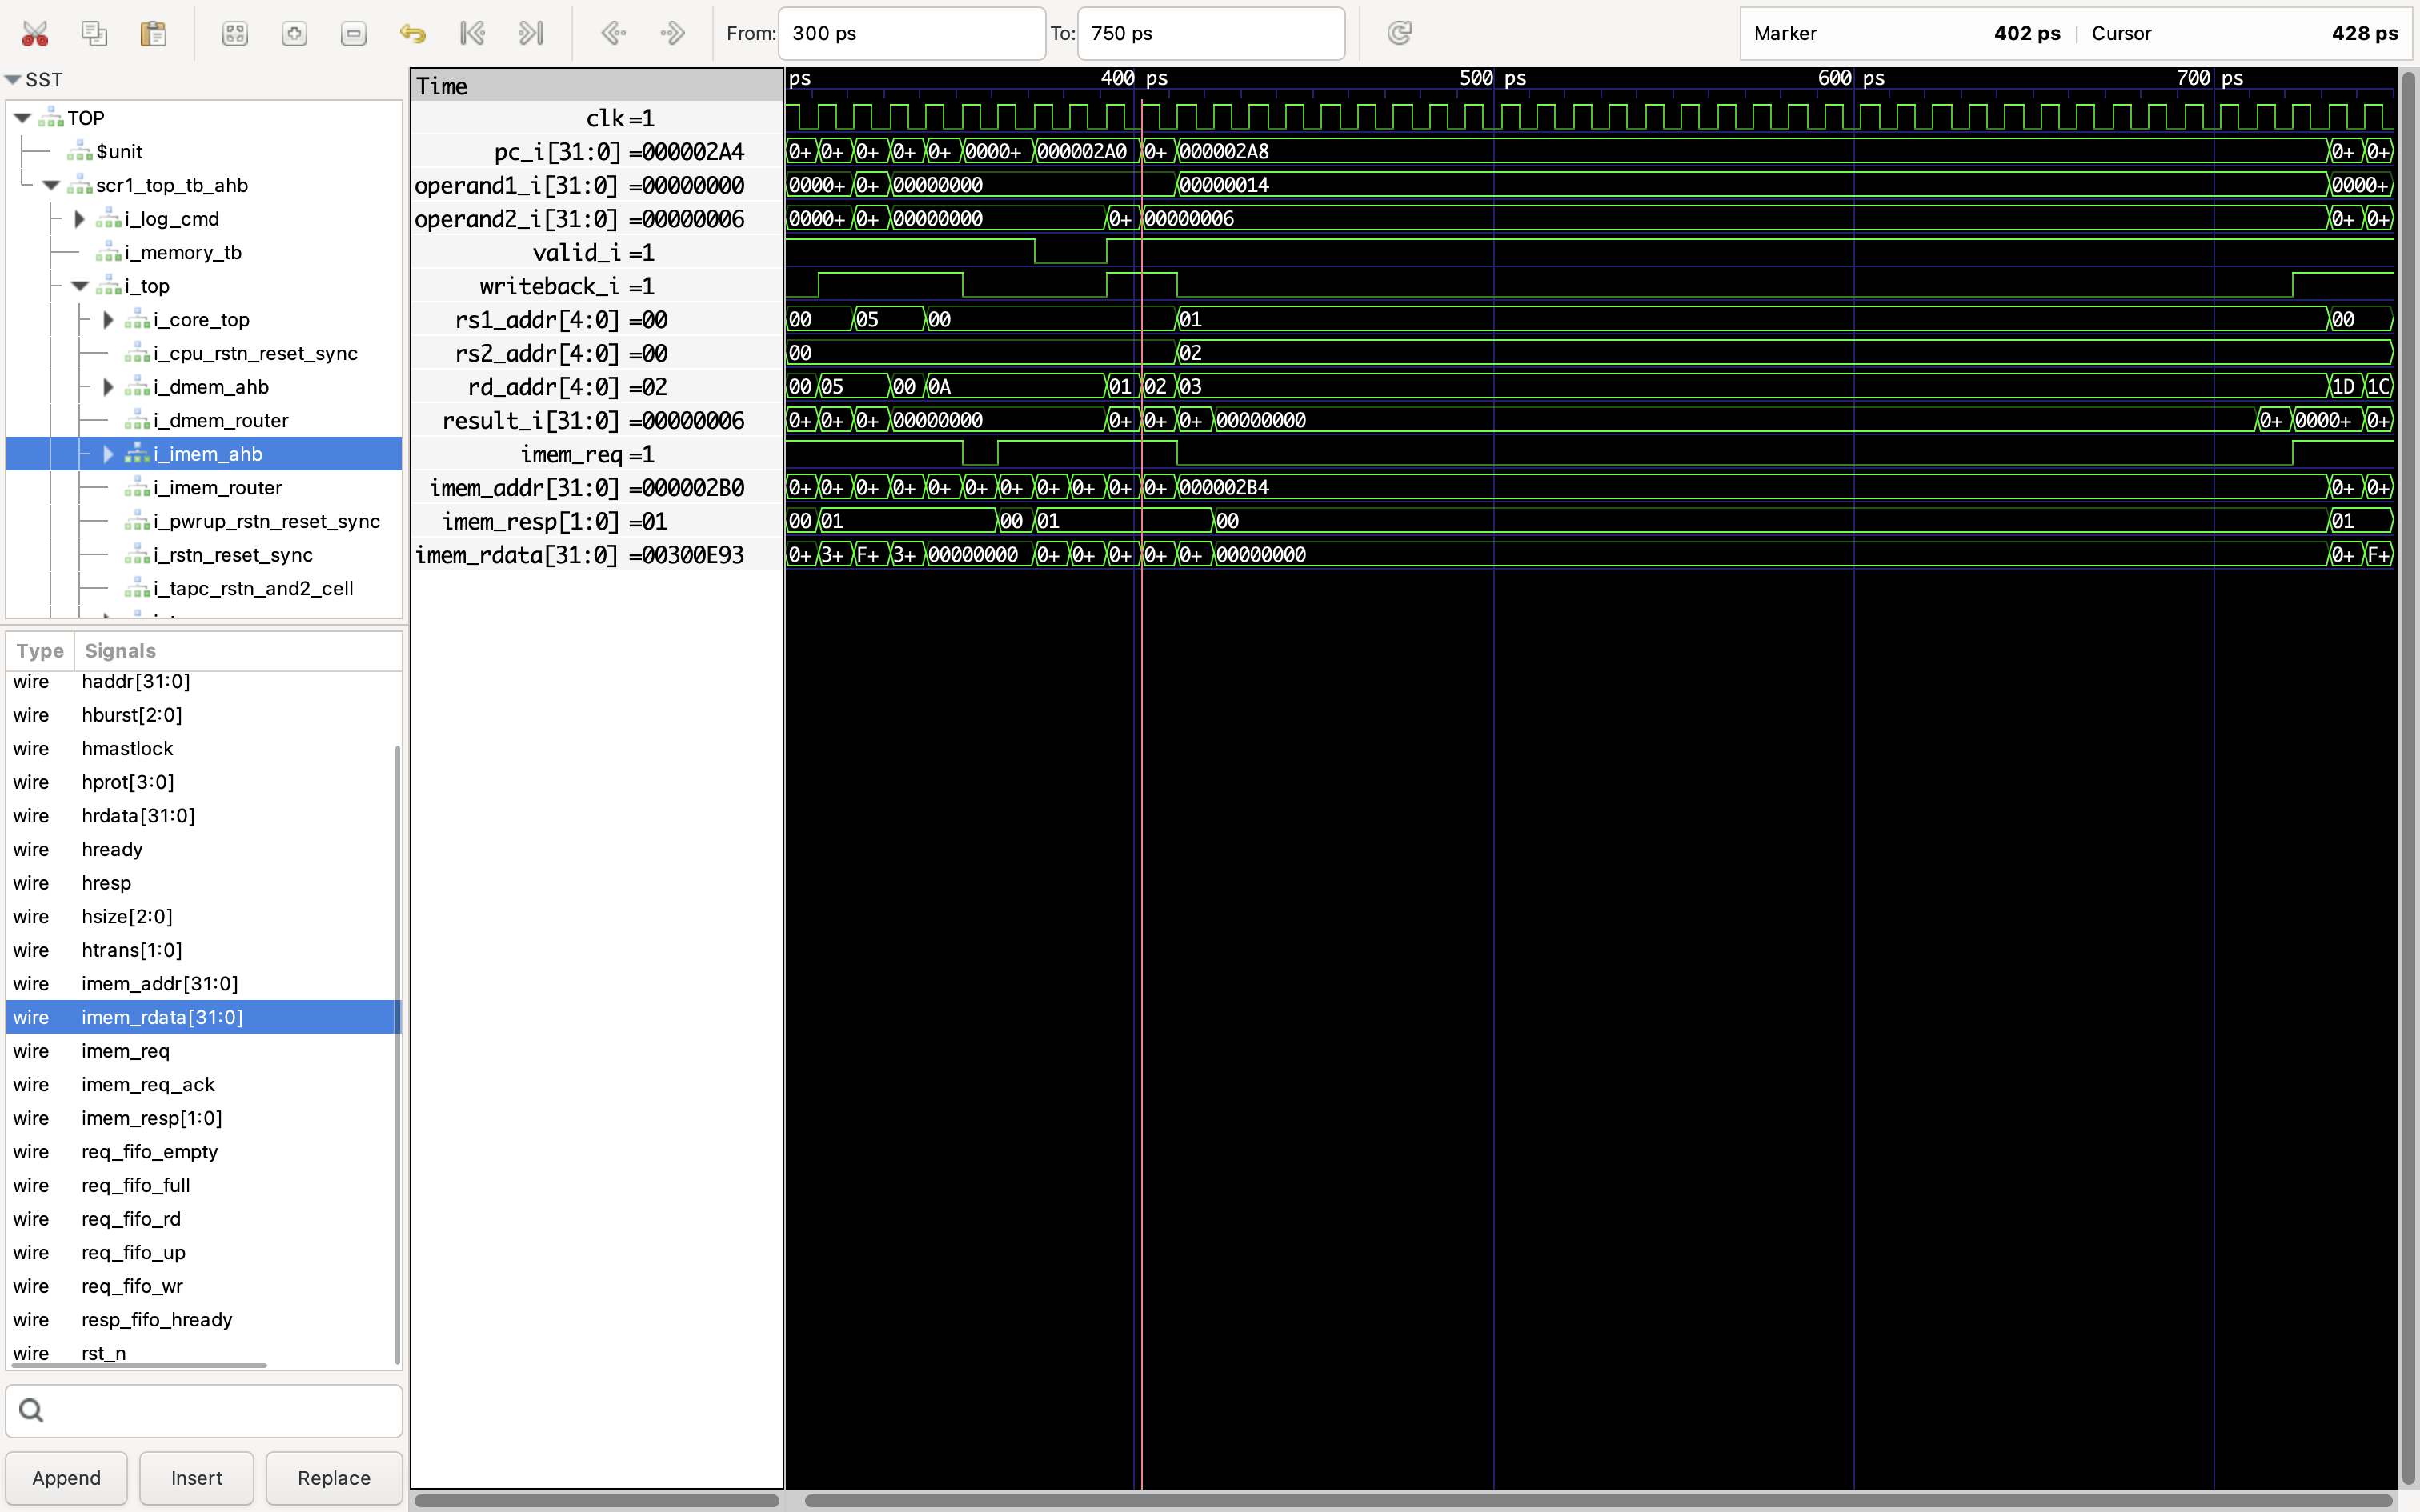
\includegraphics[width=\linewidth,trim={255bp 585bp 13bp 41bp},clip]{diagram.png}
\caption{Скриншот GTKWave: исполнение DIV по адресу 0x2A8,
операнды 0x14 и 0x06, регистры x1, x2 и x3.}
\label{fig:gtkwave-div}
\end{figure}

На скриншоте значения после знака равенства слева от графиков относятся
к позиции маркера, а не ко всему интервалу. Команду DIV следует
идентифицировать по участку \texttt{pc\_i = 0x2A8} при
\texttt{valid\_i = 1}; её результат учитывается при разрешённой записи.

Следующие поясняющие диаграммы сохраняют реальные времена и значения
той же трассы. Адреса и данные инструкций показаны в шестнадцатеричной
системе, операнды и арифметический результат --- в знаковой десятичной;
время --- в ps.

Включены обязательные сигналы задания: \texttt{clk}, текущий PC стадии
исполнения (в наблюдателе называется \texttt{pc\_i}),
\texttt{imem\_req}, \texttt{imem\_addr}, \texttt{imem\_resp},
\texttt{imem\_rdata}. Дополнительно показаны операнды, готовность IALU,
достоверность команды, результат и разрешение записи.

\begin{figure}
\centering
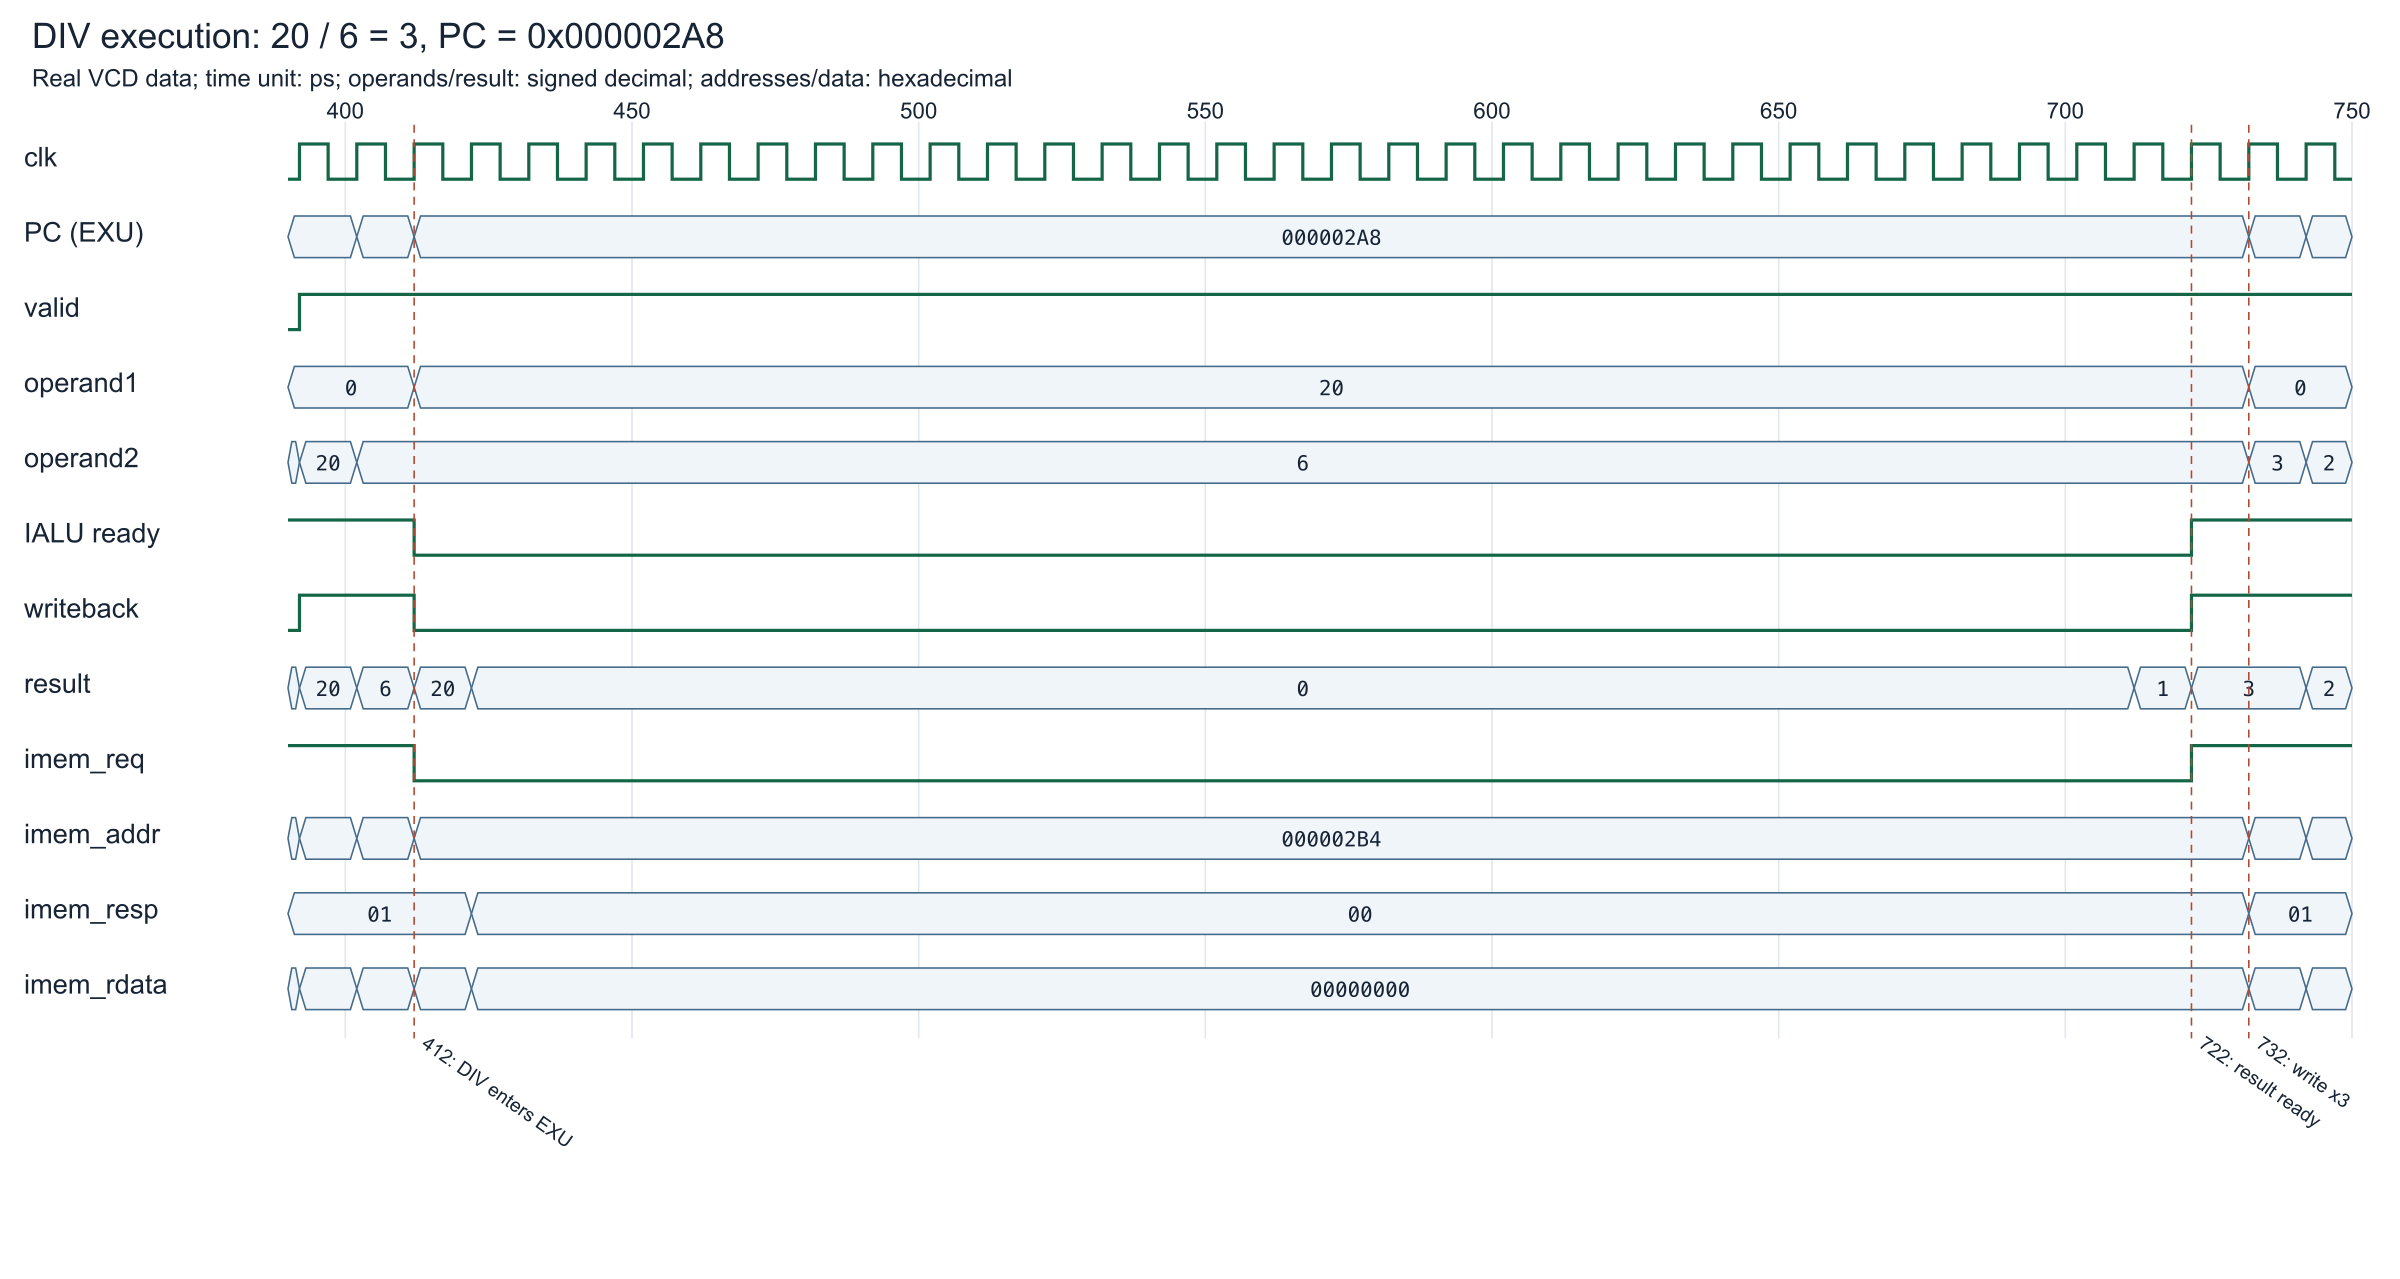
\includegraphics[width=1\linewidth,height=\textheight,keepaspectratio,alt={Исполнение первой DIV и запись результата.}]{assets/div_execution.png}
\caption{Исполнение первой DIV и запись результата.}
\end{figure}

{\def\LTcaptype{none} % do not increment counter
\begin{longtable}[]{@{}
  >{\raggedright\arraybackslash}p{(\linewidth - 2\tabcolsep) * \real{0.5000}}
  >{\raggedright\arraybackslash}p{(\linewidth - 2\tabcolsep) * \real{0.5000}}@{}}
\toprule\noalign{}
\begin{minipage}[b]{\linewidth}\raggedright
Время, ps
\end{minipage} & \begin{minipage}[b]{\linewidth}\raggedright
Наблюдаемое событие
\end{minipage} \\
\midrule\noalign{}
\endhead
\bottomrule\noalign{}
\endlastfoot
412 & PC исполнения принимает значение 0x2A8. Операнды равны 0x14 (20) и
0x06 (6). Готовность и разрешение записи опускаются. \\
412--722 & Команда удерживается в EXU, вычисление продолжается.
Промежуточное значение результата нельзя считать готовым частным. \\
722 & IALU выдаёт готовность. Результат равен 3, запись разрешена. \\
732 & На положительном фронте число 3 записывается в x3. Наблюдатель
печатает сообщение. PC переходит к 0x2AC. \\
\end{longtable}
}

Период такта в трассе --- 10 ps. Интервал от приёма команды до фронта
записи составляет 732 − 412 = 320 ps, то есть 32 тактовых периода для
выбранной операции. Это модельное время RTL-симуляции, а не оценка
допустимой частоты реального кристалла.

\begin{figure}
\centering
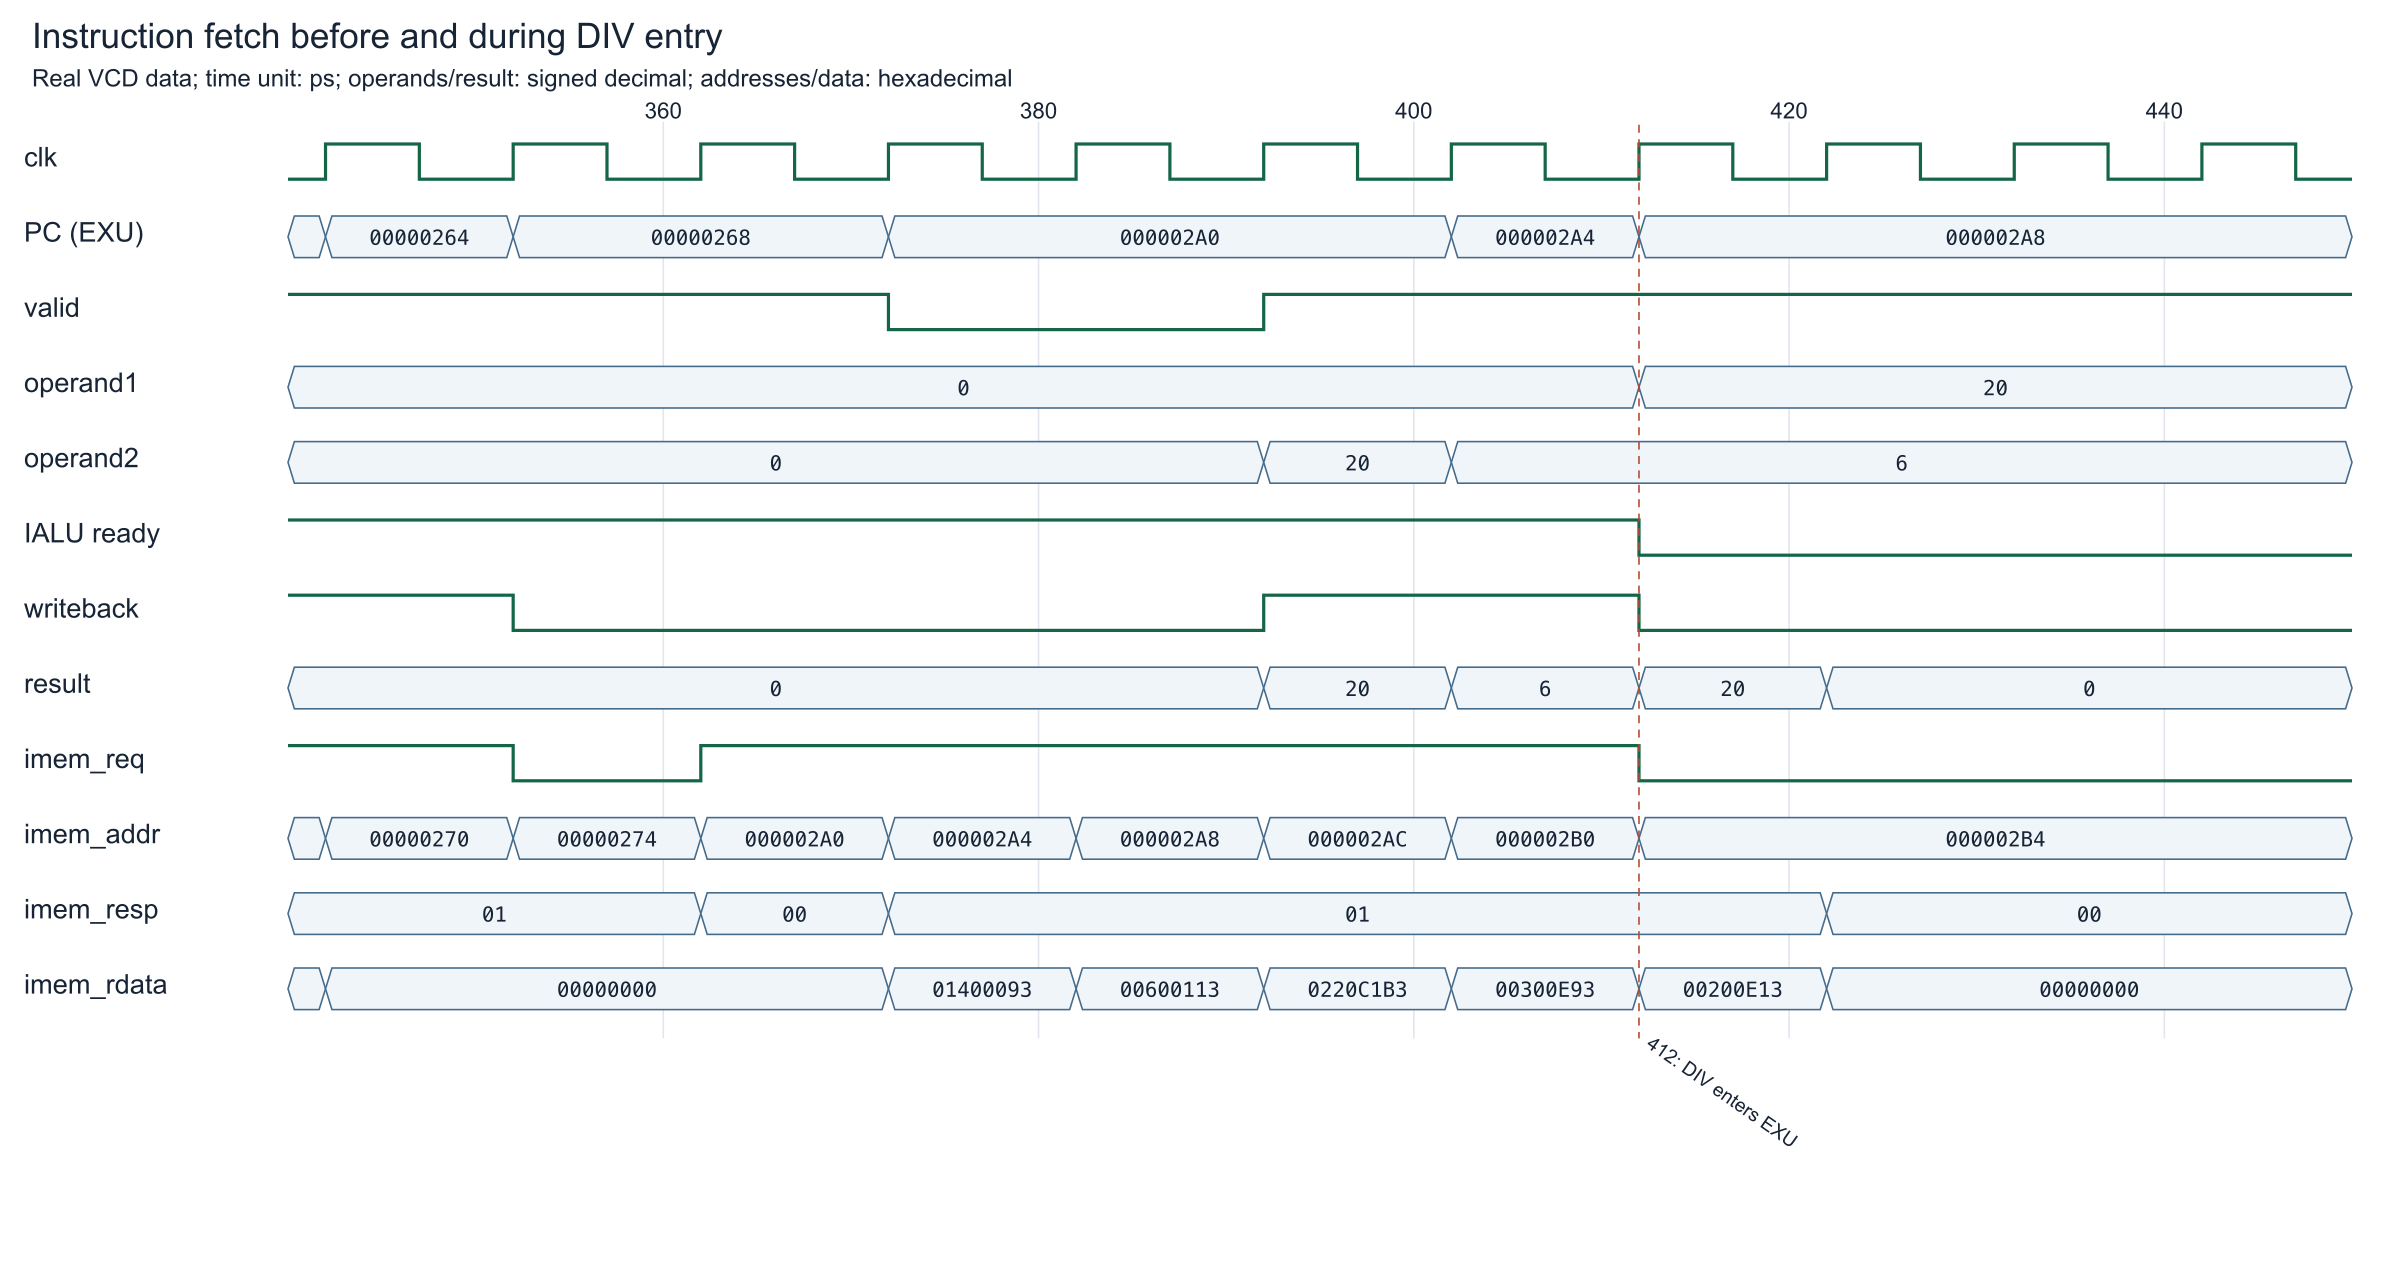
\includegraphics[width=1\linewidth,height=\textheight,keepaspectratio,alt={Интерфейс выборки в окрестности поступления DIV в EXU.}]{assets/div_fetch.png}
\caption{Интерфейс выборки в окрестности поступления DIV в EXU.}
\end{figure}

Выборка инструкций опережает исполнение: при PC исполнения 0x2A8
интерфейс памяти может обращаться к последующим адресам. В частности,
код 0x00200E13 соответствует \texttt{li\ x28,\ 2} по адресу 0x2B0, а не
DIV.

Данные \texttt{imem\_rdata} трактуются как достоверная инструкция при
успешном ответе \texttt{imem\_resp\ =\ 01}. При
\texttt{imem\_resp\ =\ 00} готового ответа нет; нулевые данные на шине в
это время не означают выполнение нулевой инструкции. Значение
\texttt{imem\_addr} без принятого запроса также не означает новую
выборку.

\section{7. Результаты
проверки}\label{ux440ux435ux437ux443ux43bux44cux442ux430ux442ux44b-ux43fux440ux43eux432ux435ux440ux43aux438}

Симуляция завершилась результатом \textbf{1/1 tests passed},
\texttt{div.hex\ —\ OK,\ PASS}. Наблюдатель вывел девять операций,
полный вывод сохранён в \texttt{report/div\_debug.log}.

{\def\LTcaptype{none} % do not increment counter
\begin{longtable}[]{@{}lrrr@{}}
\toprule\noalign{}
PC & Делимое & Делитель & Частное \\
\midrule\noalign{}
\endhead
\bottomrule\noalign{}
\endlastfoot
0x2A8 & 20 & 6 & 3 \\
0x2C0 & -20 & 6 & -3 \\
0x2D8 & 20 & -6 & -3 \\
0x2F0 & -20 & -6 & 3 \\
0x308 & -2147483648 & 1 & -2147483648 \\
0x320 & -2147483648 & -1 & -2147483648 \\
0x338 & -2147483648 & 0 & -1 \\
0x350 & 1 & 0 & -1 \\
0x368 & 0 & 0 & -1 \\
\end{longtable}
}

Проверены разные сочетания знаков, граничное отрицательное значение и
деление на ноль. Для DIV деление на ноль даёт все единицы в результате
(−1 при знаковом отображении), а переполнение −2147483648 / −1 даёт
−2147483648. Эти случаи не вызывают исключения деления на ноль или
переполнения.


Пример фактической строки вывода наблюдателя (первая операция):

{\scriptsize
\begin{verbatim}
[DIV] PC=0x000002a8 rs1=x1 rs2=x2 rd=x3 operand1=20 operand2=6 result=3
\end{verbatim}
}

Номер регистра результата \texttt{rd=x3} и значение \texttt{result=3}
здесь совпадают численно случайно: первое указывает место записи,
второе является вычисленным частным. Вывод сделан на фронте записи
результата, а не при выборке машинного слова из памяти.

Наблюдатель выводит данные, а правильность результата проверяет
программа ISA-теста. Адреса всех девяти сообщений сопоставлены с
инструкциями DIV в \texttt{div.dump}.

\section{8. Вывод}\label{ux432ux44bux432ux43eux434}

Исследован путь DIV от декодирования до записи частного в регистр.
Добавлен несинтезируемый наблюдатель, выводящий атрибуты завершённой
инструкции. Для операции 20 / 6 подтверждены PC 0x2A8, источники x1 и
x2, результат 3 в x3 и длительность пребывания команды в EXU 32 периода
такта. Тест завершился успешно.

\section{9. Использованные
материалы}\label{ux438ux441ux43fux43eux43bux44cux437ux43eux432ux430ux43dux43dux44bux435-ux43cux430ux442ux435ux440ux438ux430ux43bux44b}

\begin{itemize}
\tightlist
\item
  Методические указания «Лабораторная работа 3», пункты задания и
  вариант 9.
\item
  Исходные файлы SCR1: \texttt{scr1\_pipe\_idu.sv},
  \texttt{scr1\_pipe\_exu.sv}, \texttt{scr1\_pipe\_ialu.sv},
  \texttt{scr1\_pipe\_mprf.sv}.
\item
  Результаты текущего запуска: \texttt{div.dump}, \texttt{simx.vcd},
  \texttt{test\_results.txt}, \texttt{report/div\_debug.log}.
\end{itemize}


\section{10. Итог выполнения задания}

\begin{enumerate}
\item Создана отдельная ветка \texttt{lab3\_scr1\_pipe\_analys}.
\item Выбран и запущен единственный тест \texttt{isa/rv32um/div.S}.
Симуляция завершилась результатом \texttt{PASS}.
\item Исследовано выполнение DIV в конвейере. На диаграмму выведены
обязательные сигналы и дополнительные данные для анализа операндов,
готовности и записи результата.
\item Добавлен несинтезируемый наблюдатель \texttt{scr1\_tb\_log\_cmd}.
Его вывод содержит адрес команды, номера регистров, значения операндов
и вычисленное частное. Получено девять сообщений о завершённых DIV.
\item В папке \texttt{report/} подготовлены отчёт, скриншот GTKWave,
поясняющие диаграммы, текстовый вывод наблюдателя и результат теста.
\item Изменения исходников зафиксированы коммитом
\texttt{60646bb} (\texttt{Add simulation}); ветка с реализацией
отправлена в личный репозиторий GitHub.
\end{enumerate}

Для повторной сборки отчёта из папки \texttt{report/} используется:

\begin{verbatim}
xelatex lab3_report.tex
\end{verbatim}

Исходник LaTeX использует \texttt{diagram.png} и изображения
из \texttt{assets/}. Папка сгенерированной модели \texttt{build/}
для чтения отчёта не требуется.

\end{document}
